% interactcadsample.tex
% v1.04 - May 2023

\documentclass[]{interact}

\usepackage{epstopdf}% To incorporate .eps illustrations using PDFLaTeX, etc.
\usepackage{subfigure}% Support for small, `sub' figures and tables
%\usepackage[nolists,tablesfirst]{endfloat}% To `separate' figures and tables from text if required

\usepackage{natbib}% Citation support using natbib.sty
\bibpunct[, ]{(}{)}{;}{a}{}{,}% Citation support using natbib.sty
\renewcommand\bibfont{\fontsize{10}{12}\selectfont}% Bibliography support using natbib.sty

\theoremstyle{plain}% Theorem-like structures provided by amsthm.sty
\newtheorem{theorem}{Theorem}[section]
\newtheorem{lemma}[theorem]{Lemma}
\newtheorem{corollary}[theorem]{Corollary}
\newtheorem{proposition}[theorem]{Proposition}

\theoremstyle{definition}
\newtheorem{definition}[theorem]{Definition}
\newtheorem{example}[theorem]{Example}

\theoremstyle{remark}
\newtheorem{remark}{Remark}
\newtheorem{notation}{Notation}


% tightlist command for lists without linebreak
\providecommand{\tightlist}{%
  \setlength{\itemsep}{0pt}\setlength{\parskip}{0pt}}



\usepackage{lscape}
\usepackage{hyperref}
\usepackage[utf8]{inputenc}
\def\tightlist{}
\usepackage{setspace}
\doublespacing

\usepackage{booktabs}
\usepackage{longtable}
\usepackage{array}
\usepackage{multirow}
\usepackage{wrapfig}
\usepackage{float}
\usepackage{colortbl}
\usepackage{pdflscape}
\usepackage{tabu}
\usepackage{threeparttable}
\usepackage{threeparttablex}
\usepackage[normalem]{ulem}
\usepackage{makecell}
\usepackage{xcolor}

\begin{document}


\articletype{}

\title{Appendix to ``Automated Assessment of Residual Plots with
Computer Vision Models''}


\author{\name{Weihao Li$^{a, b}$, Dianne Cook$^{a}$, Emi Tanaka$^{a, b,
c}$, Susan VanderPlas$^{d}$, Klaus Ackermann$^{a}$}
\affil{$^{a}$Department of Econometrics and Business Statistics, Monash
University, Clayton, VIC, Australia; $^{b}$Biological Data Science
Institute, Australian National University, Acton, ACT,
Australia; $^{c}$Research School of Finance, Actuarial Studies and
Statistics, Australian National University, Acton, ACT,
Australia; $^{d}$Department of Statistics, University of Nebraska,
Lincoln, Nebraska, USA}
}


\maketitle



\appendix

\section{Data Generation}\label{sec-model-data-generation}

\subsection{Simulation Scheme}\label{simulation-scheme}

While observational data is frequently employed in training models for
real-world applications, the data generating process of observational
data often remains unknown, making computation for our target variable
\(D\) unattainable. Consequently, the computer vision models developed
in this study were trained using synthetic data, including 80,000
training images and 8,000 test images. This approach provided us with
precise label annotations. Additionally, it ensured a large and diverse
training dataset, as we had control over the data generating process,
and the simulation of the training data was relatively cost-effective.

We have incorporated three types of residual departures of linear
regression model in the training data, including non-linearity,
heteroskedasticity and non-normality. All three departures can be
summarized by the data generating process formulated as

\begin{align} \label{eq:data-sim}
\boldsymbol{y} &= \boldsymbol{1}_n + \boldsymbol{x}_1 + \beta_1\boldsymbol{x}_2 + \beta_2(\boldsymbol{z} + \beta_1\boldsymbol{w}) + \boldsymbol{k} \odot \boldsymbol{\varepsilon}, \\
\boldsymbol{z} &= \text{He}_j(g(\boldsymbol{x}_1, 2)), \\
\boldsymbol{w} &= \text{He}_j(g(\boldsymbol{x}_2, 2)), \\
\boldsymbol{k} &= \left[\boldsymbol{1}_n + b(2 - |a|)(\boldsymbol{x}_1 + \beta_1\boldsymbol{x}_2 - a\boldsymbol{1}_n)^{\circ2}\right]^{\circ1/2},
\end{align}

\noindent where \(\boldsymbol{y}\), \(\boldsymbol{x}_1\),
\(\boldsymbol{x}_2\), \(\boldsymbol{z}\), \(\boldsymbol{w}\),
\(\boldsymbol{k}\) and \(\boldsymbol{\varepsilon}\) are vectors of size
\(n\), \(\boldsymbol{1}_n\) is a vector of ones of size \(n\),
\(\boldsymbol{x}_1\) and \(\boldsymbol{x}_2\) are two independent
predictors, \(\text{He}_j(.)\) is the \(j\)th-order probabilist's
Hermite polynomials \citep{hermite1864nouveau}, \((.)^{\circ2}\) and
\((.)^{\circ1/2}\) are Hadamard square and square root, \(\odot\) is the
Hadamard product, and \(g(\boldsymbol{x}, k)\) is a scaling function to
enforce the support of the random vector to be \([-k, k]^n\) defined as

\[g(\boldsymbol{x}, k) = 2k \cdot \frac{\boldsymbol{x} - x_{\min}\boldsymbol{1}_n}{x_{\max} - x_{\min}} - k\boldsymbol{1}_n,~for~k > 0,\]
\noindent where \(x_{\min} = \underset{i \in \{ 1,...,n\}}{\min} x_i\),
\(x_{\max} = \underset{i \in \{ 1,...,n\}}{\max} x_i\) and \(x_i\) is
the \(i\)-th entry of \(\boldsymbol{x}\).

\begin{table}

\caption{\label{tab:factor}Factors used in the data generating process for synthetic data simulation. Factor $j$ and $a$ controls the non-linearity shape and the heteroskedasticity shape respectively. Factor $b$, $\sigma_\varepsilon$ and $n$ control the signal strength. Factor $\text{dist}_\varepsilon$, $\text{dist}_{x1}$ and $\text{dist}_{x2}$ specifies the distribution of $\varepsilon$, $X_1$ and $X_2$ respectively.}
\centering
\begin{tabular}[t]{ll}
\toprule
Factor & Domain\\
\midrule
j & \{2, 3, ..., 18\}\\
a & {}[-1, 1]\\
b & {}[0, 100]\\
$\beta_1$ & \{0, 1\}\\
$\beta_2$ & \{0, 1\}\\
\addlinespace
$\text{dist}_\varepsilon$ & \{discrete, uniform, normal, lognormal\}\\
$\text{dist}_{x1}$ & \{discrete, uniform, normal, lognormal\}\\
$\text{dist}_{x2}$ & \{discrete, uniform, normal, lognormal\}\\
$\sigma_{\varepsilon}$ & {}[0.0625, 9]\\
$\sigma_{X1}$ & {}[0.3, 0.6]\\
\addlinespace
$\sigma_{X2}$ & {}[0.3, 0.6]\\
n & {}[50, 500]\\
\bottomrule
\end{tabular}
\end{table}

The residuals and fitted values of the fitted model were obtained by
regressing \(\boldsymbol{y}\) on \(\boldsymbol{x}_1\). If
\(\beta_1 \neq 0\), \(\boldsymbol{x}_2\) was also included in the design
matrix. This data generation process was adapted from
\citet{li2024plot}, where it was utilized to simulate residual plots
exhibiting non-linearity and heteroskedasticity visual patterns for
human subject experiments. A summary of the factors utilized in Equation
\ref{eq:data-sim} is provided in Table \ref{tab:factor}.

In Equation \ref{eq:data-sim}, \(\boldsymbol{z}\) and \(\boldsymbol{w}\)
represent higher-order terms of \(\boldsymbol{x}_1\) and
\(\boldsymbol{x}_2\), respectively. If \(\beta_2 \neq 0\), the
regression model will encounter non-linearity issues. Parameter \(j\)
serves as a shape parameter that controls the number of tuning points in
the non-linear pattern. Typically, higher values of \(j\) lead to an
increase in the number of tuning points, as illustrated in Figure
\ref{fig:different-j}.

\begin{figure}[!h]

{\centering 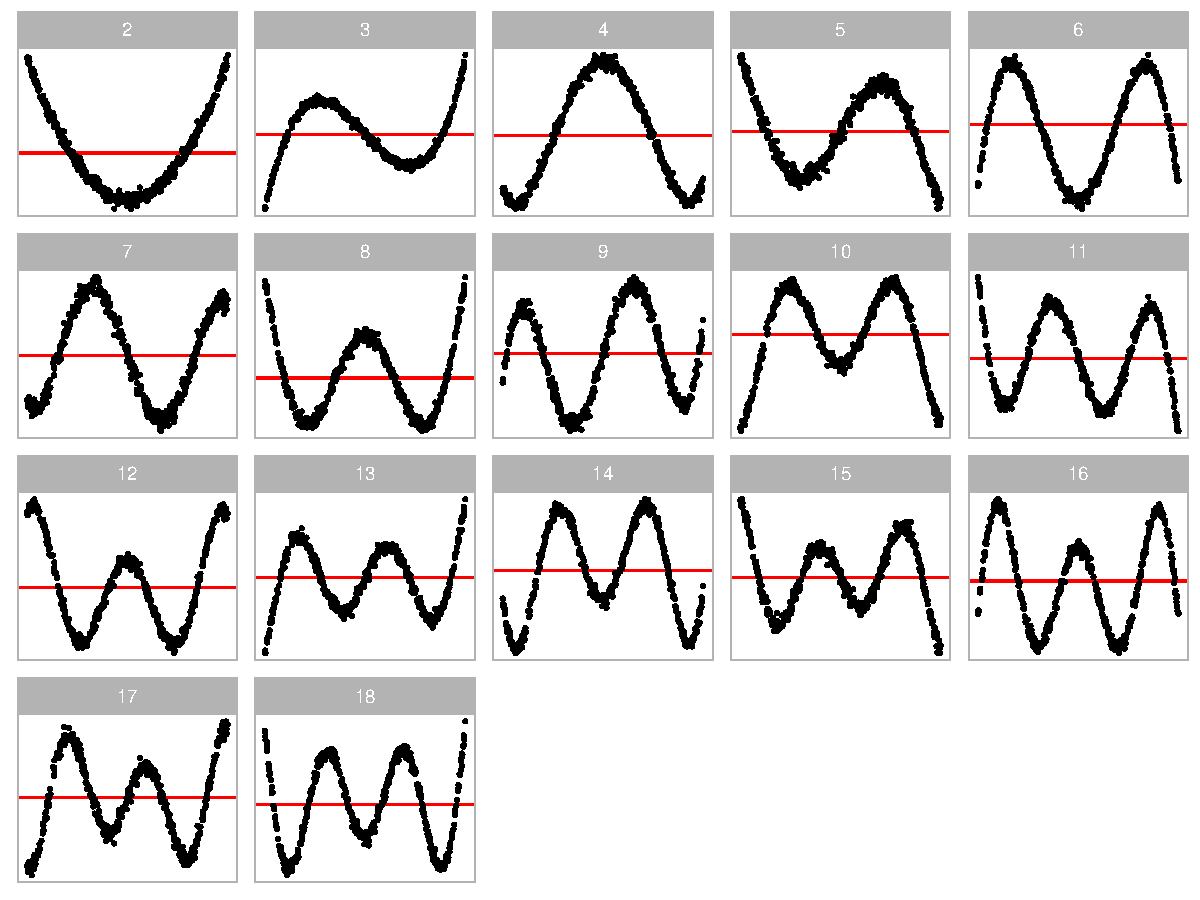
\includegraphics[width=1\linewidth]{appendix_files/figure-latex/different-j-1} 

}

\caption{Non-linearity forms generated for the synthetic data simulation. The 17 shapes are generated by varying the order of polynomial given by $j$ in $He_j(.)$.}\label{fig:different-j}
\end{figure}

Additionally, scaling factor \(\boldsymbol{k}\) directly affects the
error distribution and it is correlated with \(\boldsymbol{x}_1\) and
\(\boldsymbol{x}_2\). If \(b \neq 0\) and
\(\boldsymbol{\varepsilon} \sim N(\boldsymbol{0}_n, \sigma^2\boldsymbol{I}_n)\),
the constant variance assumption will be violated. Parameter \(a\) is a
shape parameter controlling the location of the smallest variance in a
residual plot as shown in Figure \ref{fig:different-a}.

\begin{figure}[!h]

{\centering 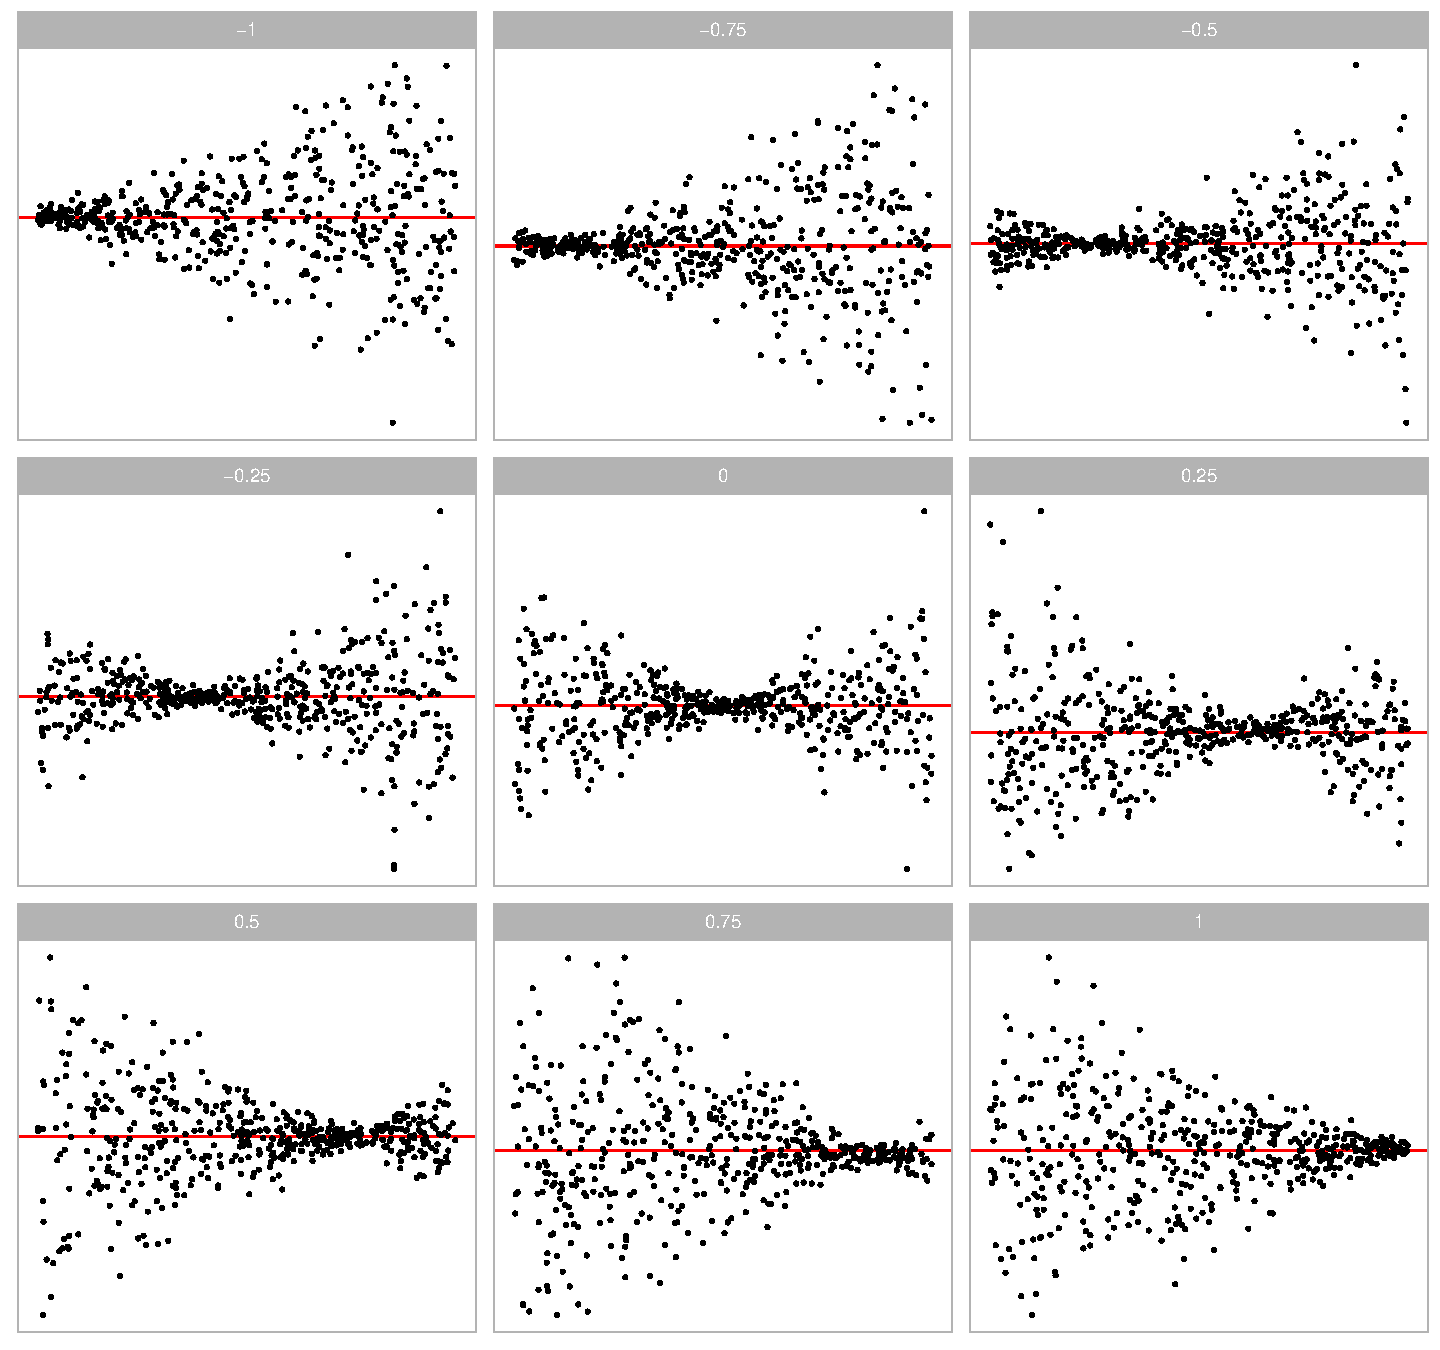
\includegraphics[width=1\linewidth]{appendix_files/figure-latex/different-a-1} 

}

\caption{Heteroskedasticity forms generated for the synthetic data simulation. Different shapes are controlled by the continuous factor $a$ between -1 and 1. For $a = -1$, the residual plot exhibits a "left-triangle" shape. And for $a = 1$, the residual plot exhibits a "right-triangle" shape. }\label{fig:different-a}
\end{figure}

\begin{figure}[!h]

{\centering 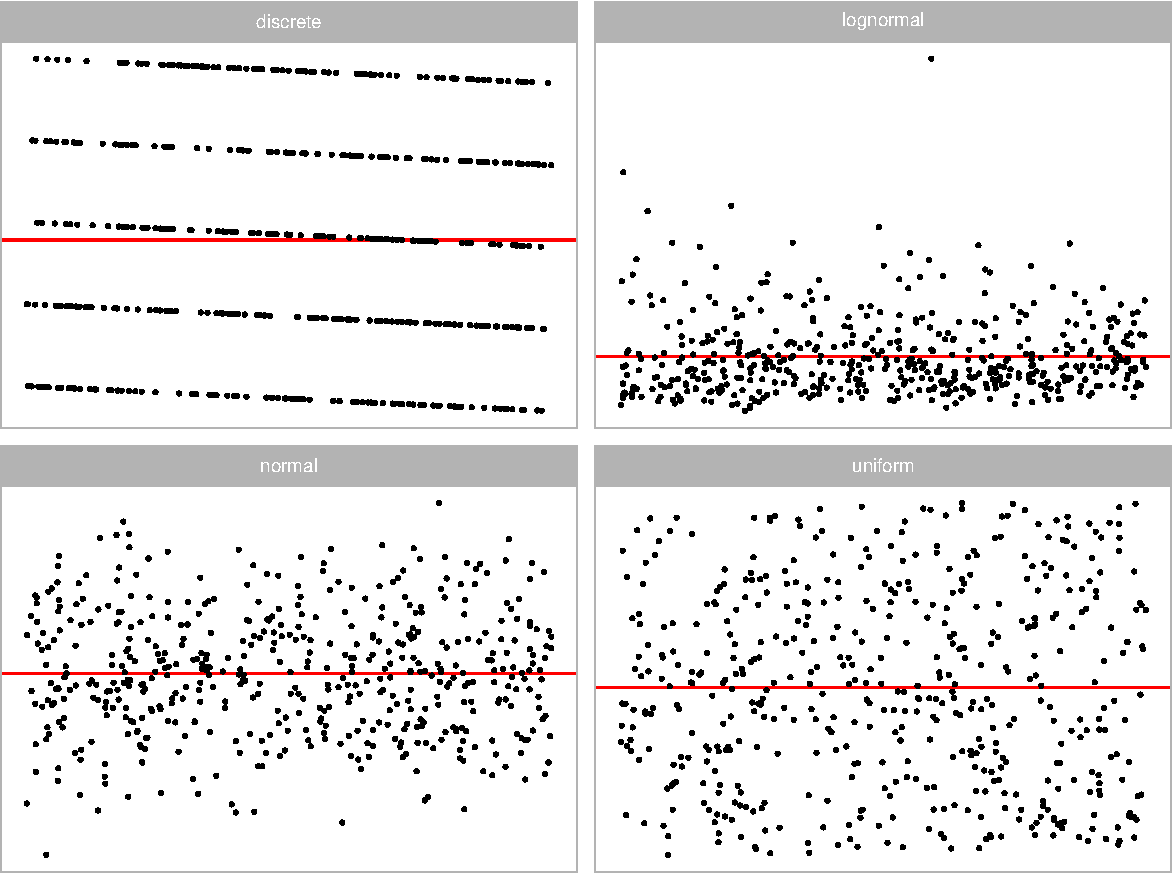
\includegraphics[width=1\linewidth]{appendix_files/figure-latex/different-e-1} 

}

\caption{Non-normality forms generated for the synthetic data simulation. Four different error distributions including discrete, lognormal, normal and uniform are considered.}\label{fig:different-e}
\end{figure}

Non-normality violations arise from specifying a non-normal distribution
for \(\boldsymbol{\varepsilon}\). In the synthetic data simulation, four
distinct error distributions are considered, including discrete,
uniform, normal, and lognormal distributions, as presented in Figure
\ref{fig:different-e}. Each distribution imparts unique characteristics
in the residual plot. The discrete error distribution introduces
discrete clusters in residuals, while the lognormal distribution
typically yields outliers. Uniform error distribution may result in
residuals filling the entire space of the residual plot. All of these
distributions exhibit visual distinctions from the normal error
distribution.

\begin{figure}[!h]

{\centering 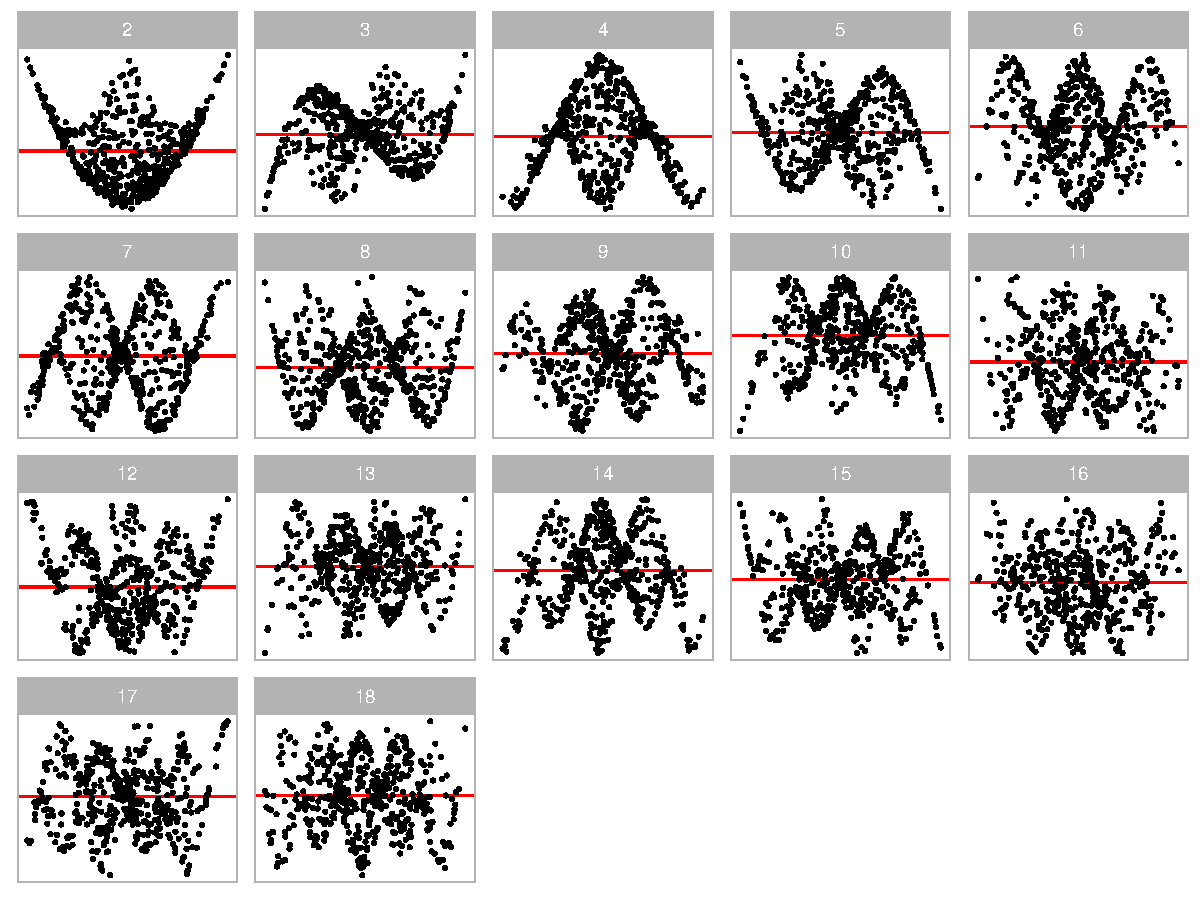
\includegraphics[width=1\linewidth]{appendix_files/figure-latex/different-j-x2-1} 

}

\caption{Residual plots of multiple linear regression models with non-linearity issues. The 17 shapes are generated by varying the order of polynomial given by $j$ in $He_j(.)$. A second predictor $\boldsymbol{x}_2$ is introduced to the regression model to create complex shapes.}\label{fig:different-j-x2}
\end{figure}

\begin{figure}[!h]

{\centering 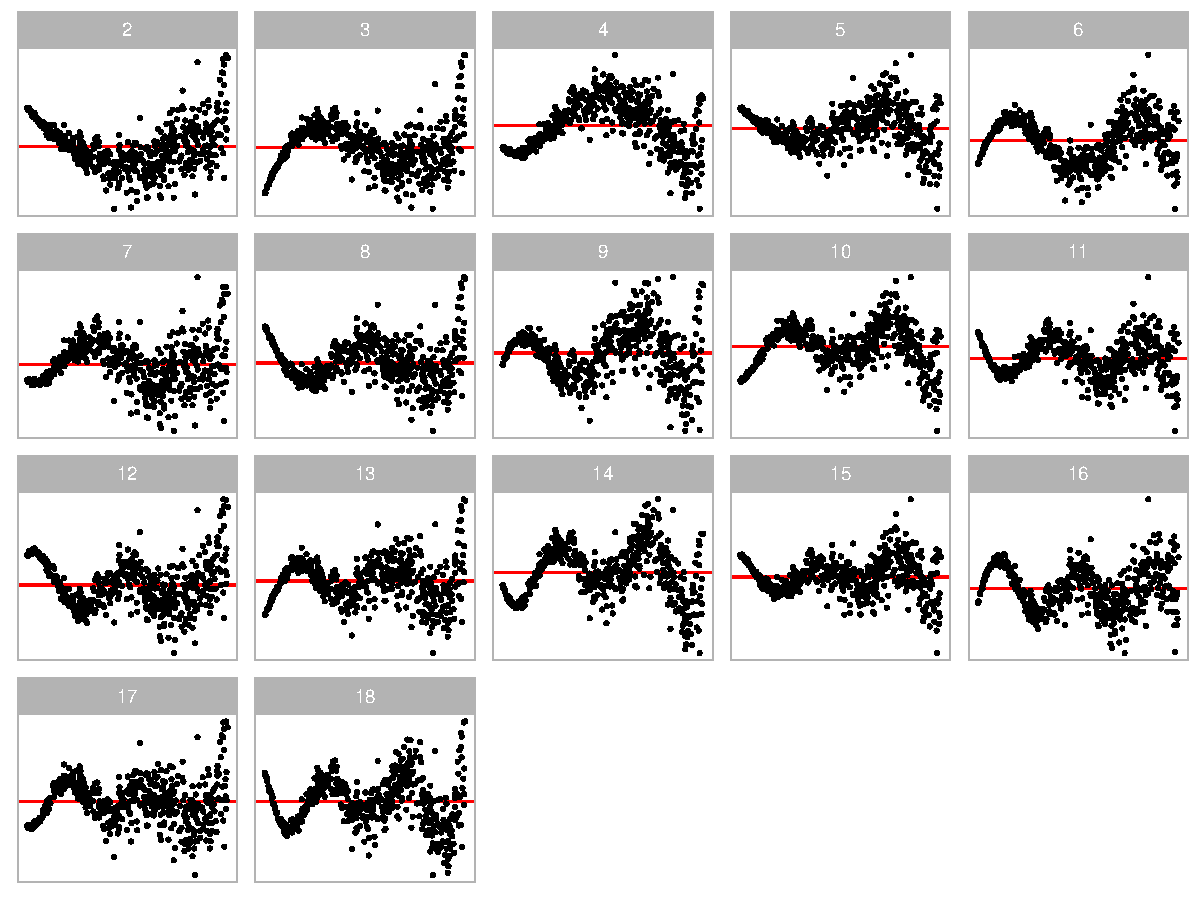
\includegraphics[width=1\linewidth]{appendix_files/figure-latex/different-j-heter-1} 

}

\caption{Residual plots of models violating both the non-linearity and the heteroskedasticity assumptions. The 17 shapes are generated by varying the order of polynomial given by $j$ in $He_j(.)$, and the "left-triangle" shape is introduced by setting $a = -1$.}\label{fig:different-j-heter}
\end{figure}

\begin{figure}[!h]

{\centering 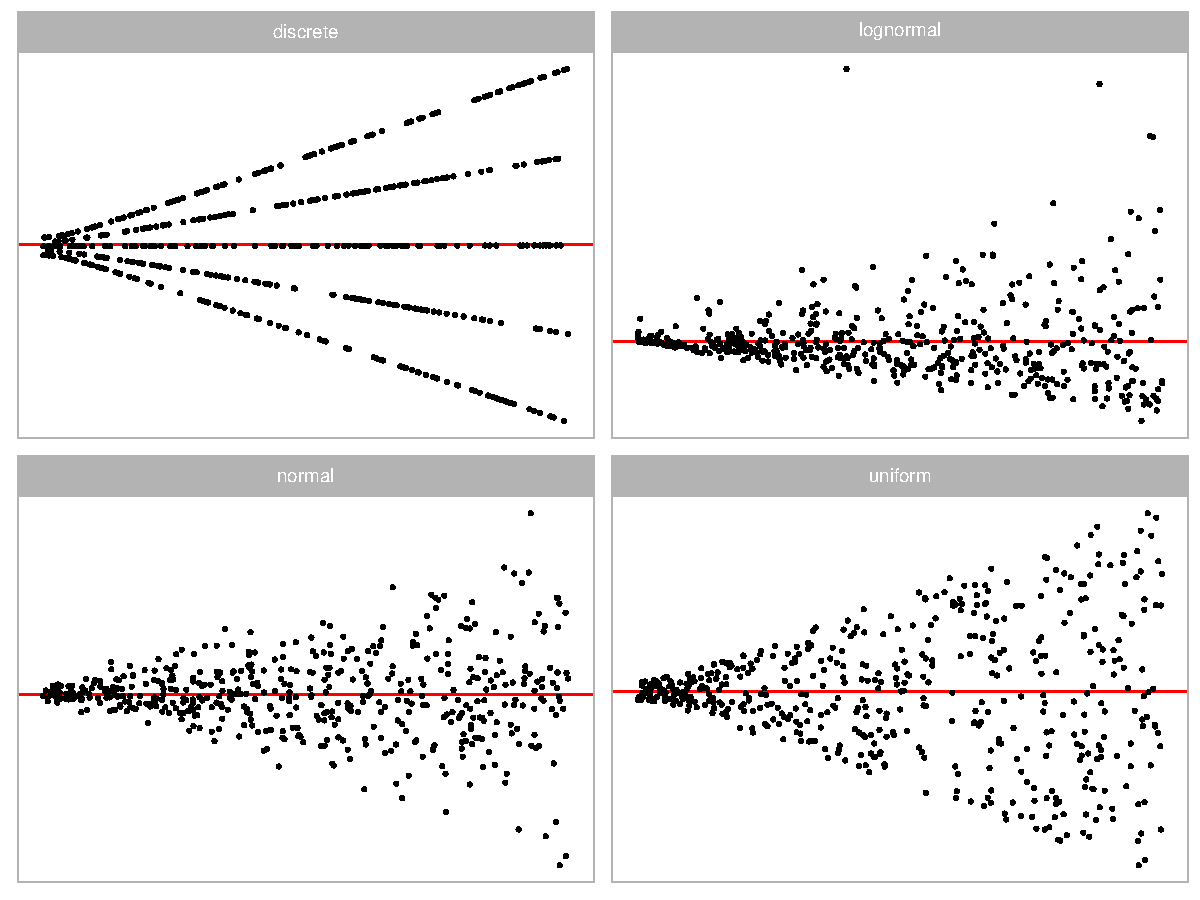
\includegraphics[width=1\linewidth]{appendix_files/figure-latex/different-e-heter-1} 

}

\caption{Residual plots of models violating both the non-normality and the heteroskedasticity assumptions. The four shapes are generated by using four different error distributions including discrete, lognormal, normal and uniform, and the "left-triangle" shape is introduced by setting $a = -1$. }\label{fig:different-e-heter}
\end{figure}

Equation \ref{eq:data-sim} accommodates the incorporation of the second
predictor \(\boldsymbol{x}_2\). Introducing it into the data generation
process by setting \(\beta_1 = 1\) significantly enhances the complexity
of the shapes, as illustrated in Figure \ref{fig:different-j-x2}. In
comparison to Figure \ref{fig:different-j}, Figure
\ref{fig:different-j-x2} demonstrates that the non-linear shape
resembles a surface rather than a single curve. This augmentation can
facilitate the computer vision model in learning visual patterns from
residual plots of the multiple linear regression model.

In real-world analysis, it is not uncommon to encounter instances where
multiple model violations coexist. In such cases, the residual plots
often exhibit a mixed pattern of visual anomalies corresponding to
different types of model violations. Figure \ref{fig:different-j-heter}
and Figure \ref{fig:different-e-heter} show the visual patterns of
models with multiple model violations.

The predictors, \(\boldsymbol{x}_1\) and \(\boldsymbol{x}_2\), are
randomly generated from four distinct distributions, including
\(U(-1, 1)\) (uniform), \(N(0, 0.3^2)\) (normal),
\(\text{lognormal}(0, 0.6^2)/3\) (skewed) and \(U\{-1, 1\}\) (discrete
uniform).

\subsection{Balanced Dataset}\label{balanced-dataset}

To train a robust computer vision model, we deliberately controlled the
distribution of the target variable \(D\) in the training data. We
ensured that it followed a uniform distribution between \(0\) and \(7\).
This was achieved by organizing \(50\) buckets, each exclusively
accepting training samples with \(D\) falling within the range
\([7(i - 1)/49, 7i/49)\) for \(i < 50\), where \(i\) represents the
index of the \(i\)-th bucket. For the \(50\)-th bucket, any training
samples with \(D \geq 7\) were accepted.

With 80,000 training images prepared, each bucket accommodated a maximum
of \(80000/ 50 = 1600\) training samples. The simulator iteratively
sampled parameter values from the parameter space, generated residuals
and fitted values using the data generation process, computed the
distance, and checked if the sample fitted within the corresponding
bucket. This process continued until all buckets were filled.

Similarly, we adopted the same methodology to prepare 8,000 test images
for performance evaluation and model diagnostics.

\section{Model Training}\label{sec-model-training}

To achieve a near-optimal deep learning model, hyperparameters like the
learning rate often need to be fine-tuned using a tuner. In our study,
we utilized the Bayesian optimization tuner from the \texttt{KerasTuner}
Python library \citep{omalley2019kerastuner} for this purpose. A
comprehensive list of hyperparameters is provided in Table
\ref{tab:hyperparameter}.

The number of base filters determines the number of filters for the
first 2D convolutional layer. In the VGG16 architecture, the number of
filters for the 2D convolutional layer in a block is typically twice the
number in the previous block, except for the last block, which maintains
the same number of convolution filters as the previous one. This
hyperparameter aids in controlling the complexity of the computer vision
model. A higher number of base filters results in more trainable
parameters. Likewise, the number of units for the fully-connected layer
determines the complexity of the final prediction block. Increasing the
number of units enhances model complexity, resulting in more trainable
parameters.

The dropout rate and batch normalization are flexible hyperparameters
that work in conjunction with other parameters to facilitate smooth
training. A higher dropout rate is necessary when the model tends to
overfit the training dataset by learning too much noise
\citep{srivastava2014dropout}. Conversely, a lower dropout rate is
preferred when the model is complex and challenging to converge. Batch
normalization, on the other hand, addresses the internal covariate shift
problem arising from the randomness in weight initialization and input
data \citep{goodfellow2016deep}. It helps stabilize and accelerate the
training process by normalizing the activations of each layer.

Additionally, incorporating additional inputs such as scagnostics and
the number of observations can potentially enhance prediction accuracy.
Therefore, we allow the tuner to determine whether these inputs were
necessary for optimal model performance.

The learning rate is a crucial hyperparameter, as it dictates the step
size of the optimization algorithm. A high learning rate can help the
model avoid local minima but risks overshooting and missing the global
minimum. Conversely, a low learning rate smoothens the training process
but makes the convergence time longer and increases the likelihood of
getting trapped in local minima.

Our model was trained on the MASSIVE M3 high-performance computing
platform \citep{goscinski2014multi}, using TensorFlow
\citep{abadi2016tensorflow} and Keras \citep{chollet2015keras}. During
training, 80\% of the training data was utilized for actual training,
while the remaining 20\% was used as validation data. The Bayesian
optimization tuner conducted 100 trials to identify the best
hyperparameter values based on validation root mean square error. The
tuner then restored the best epoch of the best model from the trials.
Additionally, we applied early stopping, terminating the training
process if the validation root mean square error fails to improve for 50
epochs. The maximum allowed epochs was set at 2,000, although no models
reached this threshold.

\begin{table}

\caption{\label{tab:hyperparameter}Name of hyperparameters and their correspoding domain for the computer vision model.}
\centering
\begin{tabular}[t]{ll}
\toprule
Hyperparameter & Domain\\
\midrule
Number of base filters & \{4, 8, 16, 32, 64\}\\
Dropout rate for convolutional blocks & {}[0.1, 0.6]\\
Batch normalization for convolutional blocks & \{false, true\}\\
Type of global pooling & \{max, average\}\\
Ignore additional inputs & \{false, true\}\\
\addlinespace
Number of units for the fully-connected layer & \{128, 256, 512, 1024, 2048\}\\
Batch normalization for the fully-connected layer & \{false, true\}\\
Dropout rate for the fully-connected layer & {}[0.1, 0.6]\\
Learning rate & {}[$10^{-8}$, $10^{-1}$]\\
\bottomrule
\end{tabular}
\end{table}

Based on the tuning process described above, the optimized
hyperparameter values are presented in Table
\ref{tab:best-hyperparameter}. It was observable that a minimum of
\(32\) base filters was necessary, with the preferable choice being
\(64\) base filters for both the \(64 \times 64\) and \(128 \times 128\)
models, mirroring the original VGG16 architecture. The optimized dropout
rate for convolutional blocks hovered around \(0.4\), and incorporating
batch normalization for convolutional blocks proved beneficial for
performance.

All optimized models chose to retain the additional inputs, contributing
to the reduction of validation error. The number of units required for
the fully-connected layer was \(256\), a relatively modest number
compared to the VGG16 classifier, suggesting that the problem at hand
was less complex. The optimized learning rates were higher for models
with higher resolution input, likely because models with more parameters
are more prone to getting stuck in local minima, requiring a higher
learning rate.

\begin{table}
\centering
\caption{\label{tab:best-hyperparameter}Hyperparameters values for the optimized computer vision models with different input sizes.}
\centering
\resizebox{\ifdim\width>\linewidth\linewidth\else\width\fi}{!}{
\begin{tabular}[t]{llll}
\toprule
Hyperparameter & $32 \times 32$ & $64 \times 64$ & $128 \times 128$\\
\midrule
Number of base filters & 32 & 64 & 64\\
Dropout rate for convolutional blocks & 0.4 & 0.3 & 0.4\\
Batch normalization for convolutional blocks & true & true & true\\
Type of global pooling & max & average & average\\
Ignore additional inputs & false & false & false\\
\addlinespace
Number of units for the fully-connected layer & 256 & 256 & 256\\
Batch normalization for the fully-connected layer & false & true & true\\
Dropout rate for the fully-connected layer & 0.2 & 0.4 & 0.1\\
Learning rate & 0.0003 & 0.0006 & 0.0052\\
\bottomrule
\end{tabular}}
\end{table}

\section{Model Violations Index}\label{sec-model-violations-index}

In Section 5.1, we noted that a pre-computed lattice of \(\hat{D}\)
quantiles can reduce the computation cost of lineup tests. Another
practical approach is to assess model performance directly using the
value of \(\hat{D}\).

The estimator \(\hat{D}\) captures the difference between the true and
reference residual distributions, which reflects the extent of model
violations, making it instrumental in forming a model violations index
(MVI). However, when more observations are used in regression, the value
of \(\hat{D}\) tends to increase logarithmically. This is because
\(D = \log(1 + D_{KL})\), and under the assumption of independence,
\(D_{KL}\) is the sum of \(D_{KL}^{(i)}\) across all observations. This
does not mean that \(\hat{D}\) becomes less reliable. In fact, larger
samples often make model violations more visible in residual plots,
unless strong overlapping masks the patterns.

However, to create a standardized and generalizable index, it is
important to adjust for the effect of sample size. Therefore, the Model
Violations Index (MVI) is proposed as

\begin{equation} \label{eq:mvi}
\text{MVI} = C + \hat{D} - \log(n),
\end{equation}

\noindent where \(C\) is a sufficiently large constant to ensure the
result remains positive, and the \(\log(n)\) term offset the increase in
\(D\) with larger sample sizes.

Figure \ref{fig:poly-heter-index} displays the residual plots for fitted
models exhibiting varying degrees of non-linearity and
heteroskedasticity. Each residual plot's MVI is computed using Equation
\ref{eq:mvi} with \(C = 10\). When \(\text{MVI} > 8\), the visual
patterns are notably strong and easily discernible by humans. In the
range \(6 < \text{MVI} < 8\), the visibility of the visual pattern
diminishes as MVI decreases. Conversely, when \(\text{MVI} < 6\), the
visual pattern tends to become relatively faint and challenging to
observe. Table \ref{tab:mvi} provides a summary of the MVI usage and it
is applicable to other linear regression models.

\begin{table}

\caption{\label{tab:mvi}Degree of model violations or the strength of the visual signals according to the Model Violations Index (MVI). The constant $C$ is set to be 10.}
\centering
\begin{tabular}[t]{lc}
\toprule
Degree of model violations & Range ($C$ = 10)\\
\midrule
Strong & $\text{MVI} > 8$\\
Moderate & $6 < \text{MVI} < 8$\\
Weak & $\text{MVI} < 6$\\
\bottomrule
\end{tabular}
\end{table}

\begin{figure}[!h]

{\centering 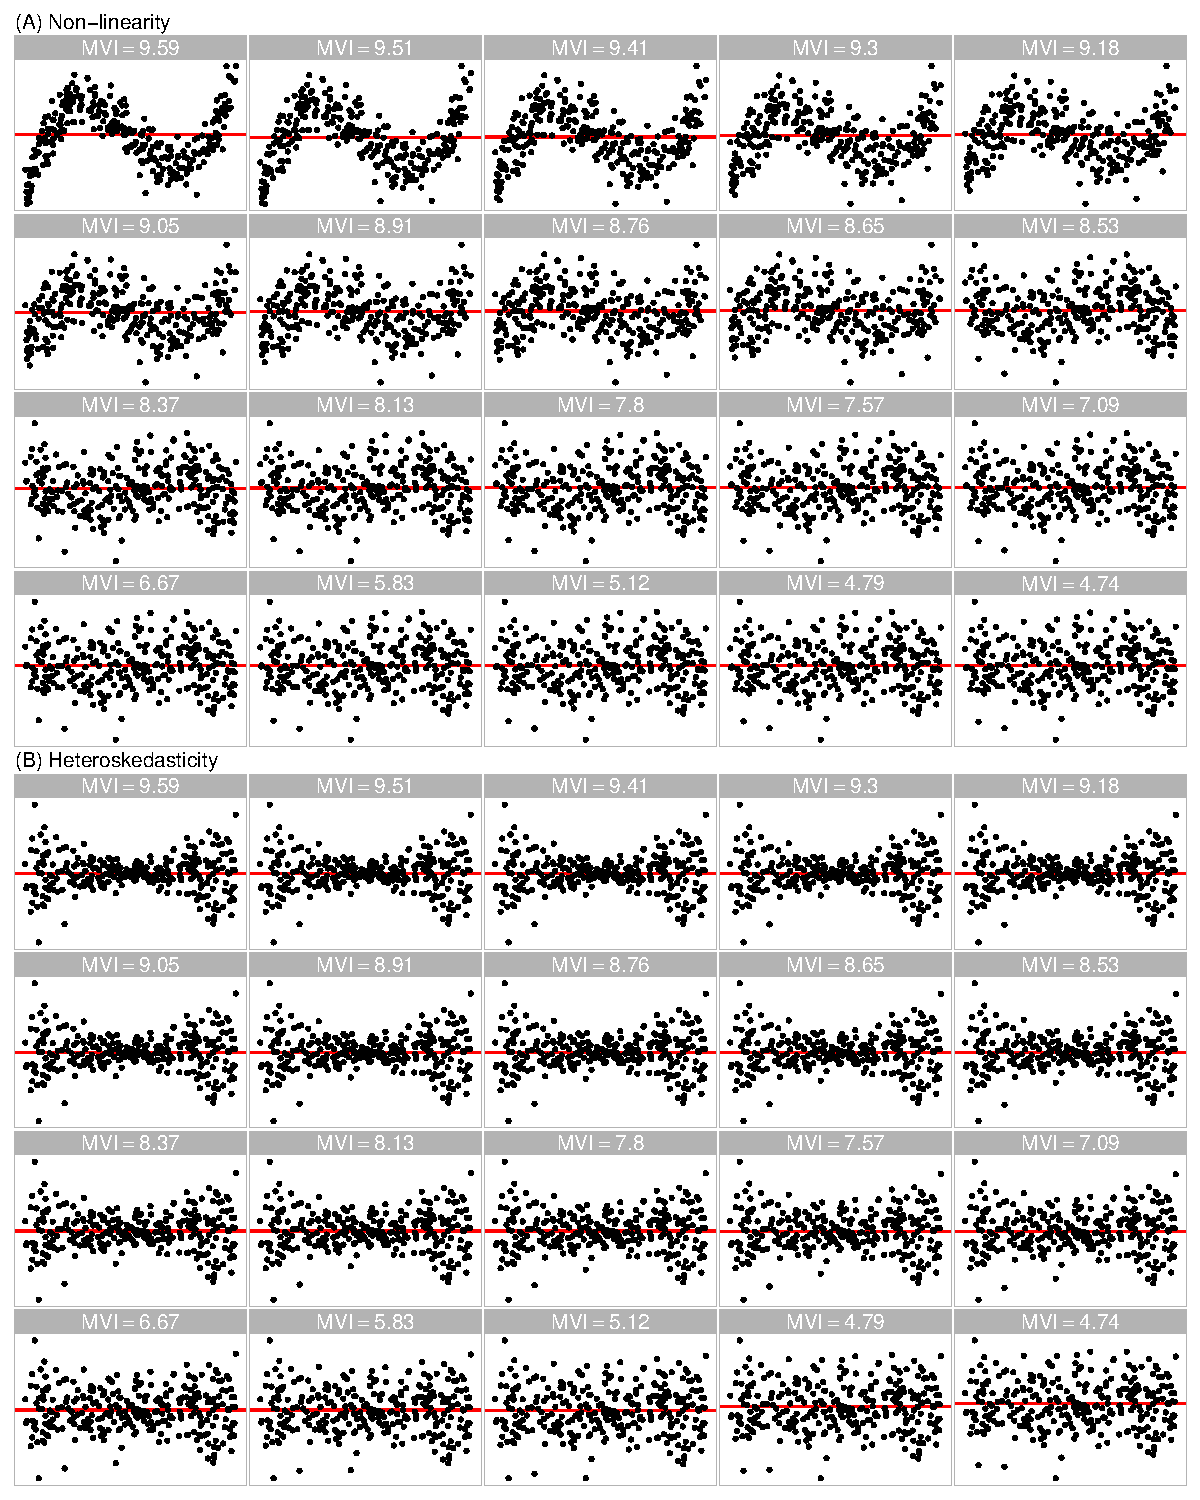
\includegraphics[width=1\linewidth]{appendix_files/figure-latex/poly-heter-index-1} 

}

\caption{Residual plots generated from fitted models exhibiting varying degrees of (A) non-linearity and (B) heteroskedasticity violations. The model violations index (MVI) is displayed atop each residual plot. The non-linearity patterns are relatively strong for $MVI > 8$, and relatively weak for $MVI < 6$, while the heteroskedasticity patterns are relatively strong for $MVI > 8$, and relatively weak for $MVI < 6$.}\label{fig:poly-heter-index}
\end{figure}

\clearpage

\bibliographystyle{tfcad}
\bibliography{bibliography.bib}





\end{document}
